%%%%%%%%%%%%%%%%%%%%%%%%%%%%%%%%%%%%%%%%%%%%%%%%%%%%%%%%%%
\section{ハミルトン閉路問題とその関連問題}\label{chap:background}
%%%%%%%%%%%%%%%%%%%%%%%%%%%%%%%%%%%%%%%%%%%%%%%%%%%%%%%%%% 

%%%%%%%%%%%%%%%%%%%%%%%%%%%%%%%%%
\begin{figure*}[t]
  \centering
  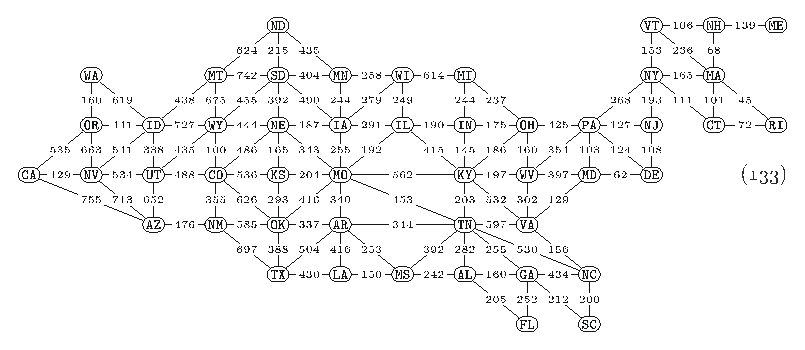
\includegraphics[width=0.7\linewidth]{fig/taocp_vol4fasc1b_p52_eq133.pdf}
  \caption{D.~E.~Knuth の教科書にある米国本土48州の隣接関係を表すグラフ}
  \label{fig:USmap}
\end{figure*}
%%%%%%%%%%%%%%%%%%%%%%%%%%%%%%%%%

グラフの全頂点を一度ずつ通る路は
\textbf{ハミルトン路}(Hamiltonian Path)と呼ばれ,
閉路は
\textbf{ハミルトン閉路}(Hamiltonian Cycle)と呼ばれる.
以下に,本稿で対象とする問題群について述べる.
\begin{itemize}
\item \textbf{ハミルトン閉路問題}は,与えられたグラフの全頂点をちょう
  ど一度ずつ通る閉路が存在するかどうかを判定する問題である.
\item \textbf{最短ハミルトン閉路問題}は,グラフの辺に距離が付随してい
  るとき,最短距離のハミルトン閉路を求める問題である.
\item \textbf{コスト制約付きハミルトン閉路問題}は,
  ハミルトン閉路問題に,距離の総和が所与の閾値以下(または以上)であるこ
  とを制約条件として付加した問題である\cite{comp20:Minato}.
\end{itemize}
これらの問題から,始点と終点が一致するという閉路の条件を取り除いた問題
を,それぞれ,ハミルトン路問題,最短ハミルトン路問題,
コスト制約付きハミルトン路問題と呼ぶ.

図~\ref{fig:USmap}は,D.~E~.Knuth の
The Art of Computer Programming~\cite{Knuth:TAOCP:BDD}
に記載されている米国本土48州の隣接関係を表すグラフである.
この隣接グラフの頂点数は48,辺の数は105である.
各辺に付与されている数字は,州都の間の距離(マイル)を表している.
西海岸ワシントン州(WA)から
東海岸メーン州(ME)までのハミルトン路は6,876,928通りあり,
最短ハミルトン路は11698マイルである.
コスト制約付きハミルトン路問題は,WA から ME までの距離の総和がある
閾値以下であるハミルトン路を求める問題と考えることができる.
本稿では,コスト制約付きハミルトン路問題の解を全列挙する問題を対象とする.
例えば,コスト制約を最短距離の10\%増(12,868マイル)以内とした場合,
解の総数は 16180 個である.

%%% Local Variables:
%%% mode: latex
%%% TeX-master: "paper"
%%% End:
